\section {First observation}

\tab Consuming alcohol and/ or smoking with some probability of getting in contact with sick persons will have a 49 per cent chance of making laringita.

\tab Some formulas ->
	\tab p(L) = p(L/al,cont) * p(al) *  p(cont) + p(L/al,-cont) * p(al) * p(-cont) =\\
		\tab	= 0.86 * 1 * 0.2 + 0.4 * 1* 0.8 = 0.172 + 0.32 = 0.492\\

\begin{center}
  	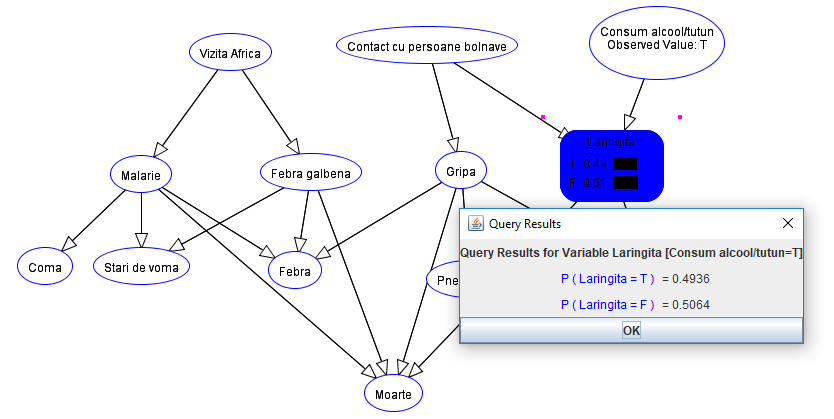
\includegraphics[scale=0.5]{p4}
\end{center}


\section{Second observation}

\tab Let's assume know that the person visited Africa, had contact with sick persons and drinks and smokes.

\begin{center}
  	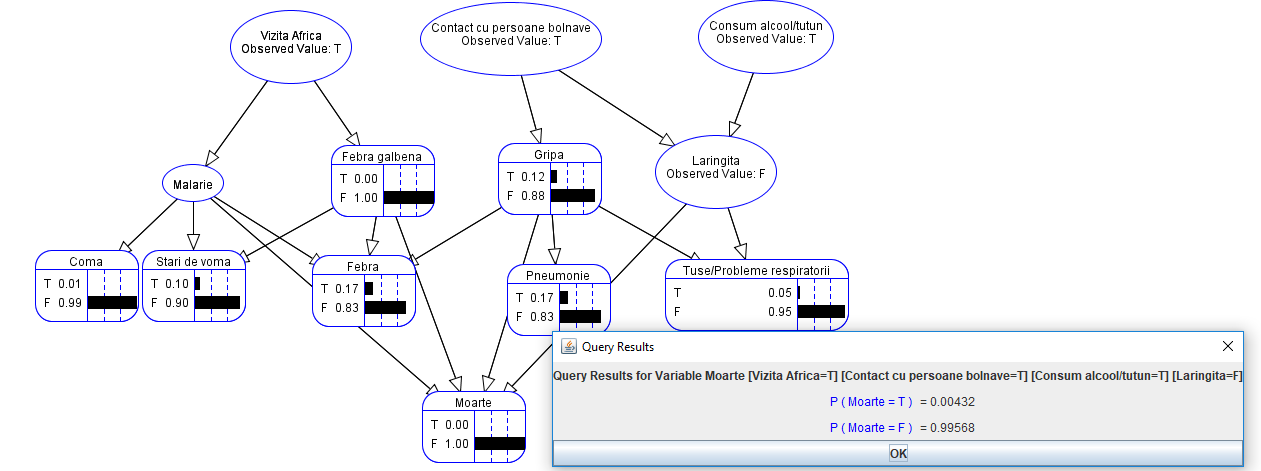
\includegraphics[scale=0.5]{p2}
\end{center}

\tab There is a 15 pc change of getting malaria-> 0.01 pc of getting a coma, it is more probable 87pc to have laryngitis. But put that all aside, what is really intresting is that the death percentage rise up to 0.00446, which is somehow bad, smoking and drinking having the biggest impact here.\\

\section {Third observation}

\tab Having malaria and yellow fever and entering a coma will bring the most likely change of getting you killed from our small percentage of statistics.. It is showing a 33pc change , which is really bad.

\begin{center}
  	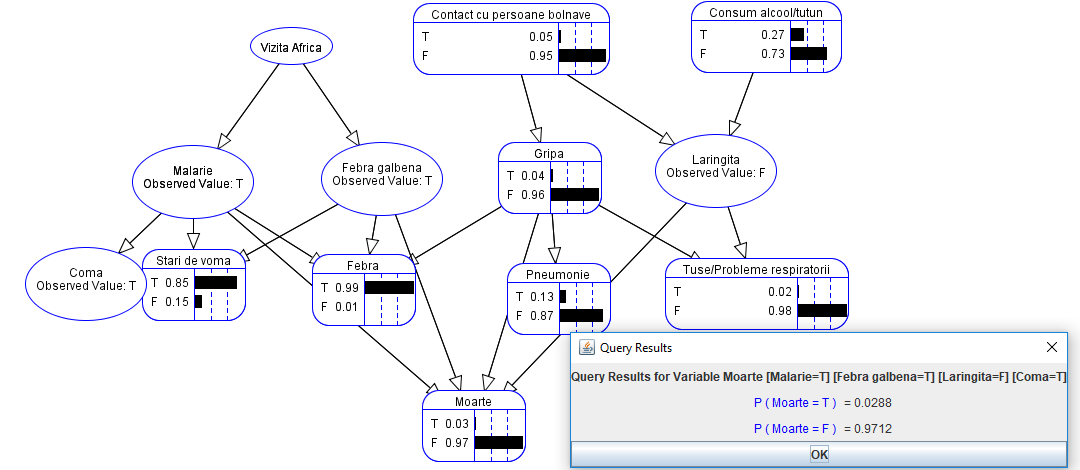
\includegraphics[scale=0.5]{p3}
\end{center}


\section{Fourth observation}

\tab We assume that a person visited africa, and got malaria and yellow fever, what is the probability of him having vomittings?, or fever, or coma? or even death? Let's find out with our first querry.\\

\begin{center}
  	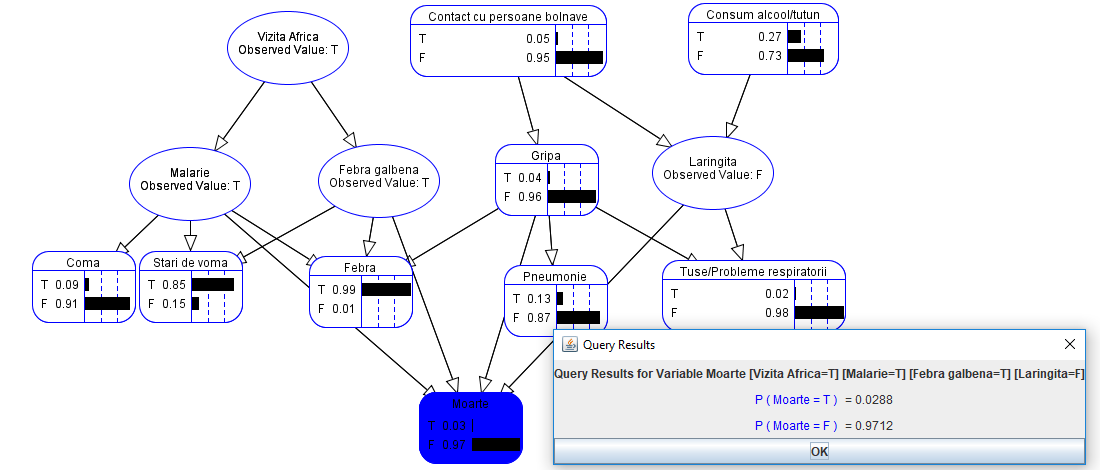
\includegraphics[scale=0.5]{p1}
\end{center}

\tab From here, we conclude that there is a 85pc change of having vomittings, 99 pc of having fever, and 0.09 pc of getting a coma, because is not that probable, and death only brings a 0.03 chance to the table. Not bad!.\\


\section{Conclusions}
\tab This project brought a lot of searching about statistics and probabilities to the table. Me and my partner
struggled to get the best available information, and filtter it. We calculated all the probabilities of the nodes
by courses formulas.\\
\tab We have some final results which can contribute to the helping of a real doctor. Of course our application can be improved
by bringing a lot more information and staticis about our nodes, but also by making it more complex.
But in it's raw stage , we can say that it can predict pretty good , based on some simptoms or first questions,
what few diseases you can have , from our small pool, and what is the percentage of some serious after effects.\\
\tab We can conlude saying that even if malaria and yellow fever are very dangerous and can cause massive damage to 
our bodies , including coma and extensive fever, the most lethal disease will remain the simple flu. Only because 
it is so widely spread accros all globe and dosen't have special requirements to get it.\\